\frame{\frametitle{Lots of open problems}
	\begin{itemize}
		\item Evaluation metrics related:
		\begin{itemize}
		\pause	\item MIRA, PRO and Perceptron require sentence level metric (BLEU doesn't work well)
		\pause	\item use good metrics
		\pause	\item but good metrics oftend are not good for tuning
		\end{itemize}
		\pause\item Representation of space of translations:
		\begin{itemize}
		\pause	\item n-best list is too small (compared to exponential space)
		\pause	\item lattice and hyper-graph are better options but too complicated to use because metrics don't decompose to (hyper-)arcs
		\pause	\item n-best is not \textit{really} n-best because of pruning which breaks convergence guarantees \cite{violation}
		\end{itemize}
		\pause \item Optimization itself:
		\pause\begin{itemize}
		\pause	\item increase margin? minimize risk?
		\pause	\item latent variables (towards which derivation to optimize?)
		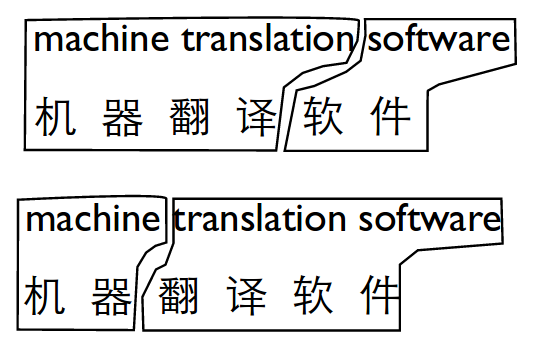
\includegraphics[width=0.30\linewidth]{MultipleDerivations}
		\end{itemize}
	\end{itemize}

}

